\documentclass{beamer}

\usepackage[T2A]{fontenc}
\usepackage[utf8x]{inputenc}
\usepackage[english,bulgarian]{babel}
\usepackage{multirow}
\usepackage{ragged2e}

\mode<presentation> {
	\usetheme{Berlin}
}

%\usebackgroundtemplate {
%	\includegraphics[width=370px, height=270px, trim=0 0 0 -80px]{background}
%}

\graphicspath{{../images/}}

\title{Въвеждане на данни и извеждане на графики}
\subtitle{Статистическа обработка на данни с R}

\author{Пламен Петров и Тодор Балабанов}

\date{12.V.2020}

\institute[ЦО и ИИКТ към БАН] {
	Център за обучение \\
	Институт по информационни и комуникационни технологии \\ 
	Българската академия на науките \\
	\medskip
	\textit{p.petrov@iit.bas.bg todorb@iinf.bas.bg}
}

\addtobeamertemplate{navigation symbols}{}{
	\usebeamerfont{footline}
	\usebeamercolor[fg]{footline}
	\hspace{1em}
	\insertframenumber/\inserttotalframenumber
}

\begin{document}

\begin{frame}
	\titlepage
\end{frame}

\begin{frame}
\begin{exampleblock}{Acknowledgments}
\justify These teaching materials are funded by Velbazhd Software LLC and it is partially supported by the Bulgarian Ministry of Education and Science (contract D01–205/23.11.2018) under the National Scientific Program ``Information and Communication Technologies for a Single Digital Market in Science, Education and Security (ICTinSES)'', approved by DCM \# 577/17.08.2018.
\end{exampleblock}
\end{frame}

\section*{Теми}
\begin{frame}[shrink]
	\frametitle{Съдържание}
	\tableofcontents
\end{frame}

\section{Работна директория}

\begin{frame}
\center \huge{Работна директория}
\end{frame}

\section{Проверка и установяване}

\begin{frame}
\frametitle{Организация на файловете}
\begin{block}{Път във файловата система}
getwd()

[1] "/Users/todorbalabanov"

setwd("~/Desktop")

getwd()

[1] "/Users/todorbalabanov/Desktop"
\end{block}
\end{frame}

\section{Структурирани източници на данни}

\begin{frame}
\center \huge{Структурирани източници на данни}
\end{frame}

\subsection{CSV файлове}

\begin{frame}
\frametitle{Текстов формат}
\begin{block}{Зареждане на данни от CSV файл}
df <- read.table(file=

$"$http://raw.githubusercontent.com/TodorBalabanov/Statistical-Data-Processing-with-R/master/data/tomato.csv$"$,

header=TRUE, sep=$"$,$"$)
\end{block}
 
\begin{block}{Оглеждане на данните}
head( df )
 
tail( df ) 

sapply(df, class)
\end{block}
\end{frame}

\subsection{Четене на данни от JSON формат}

\begin{frame}
\frametitle{JavaScript Object Notation}
\begin{block}{Четене на JSON данни}
library( jsonlite )
 
pizza <- fromJSON( $"$https://raw.githubusercontent.com/TodorBalabanov/Statistical-Data-Processing-with-R/master/data/pizza.json$"$)

class( pizza )

head(pizza, n=3)
\end{block}
\end{frame}

\subsection{Excel файлове}

\begin{frame}
\frametitle{Електронни таблици}
\begin{itemize}
	\item Четенето на Excel файлове в R не е толкова лесно
	\item Microsoft Excel е комерсиален софтуер
	\item Бинарните му файлови формати не са с отворен лиценз
	\item Има опити за четене с пакетите gdata, XLConnect, xlsReadWrite
\end{itemize}
\end{frame}

\subsection{SQL бази данни}

\begin{frame}
\frametitle{Релационни бази данни}
\begin{block}{Сваляне на файл с данни}
download.file($"$https://github.com/TodorBalabanov/Statistical-Data-Processing-with-R/blob/master/data/diamonds.db?raw=true$"$, destfile=$"$./diamonds.db$"$, mode=$"$wb$"$)
\end{block}
\end{frame}

\begin{frame}
\frametitle{Процедура за достъп}
\begin{block}{Връзка към базата данни}
library(RSQLite)

driver <- dbDriver( "SQLite" )

class( driver )

connection <- dbConnect(driver, "./diamonds.db")

class( connection )
\end{block}

\begin{block}{Комадна за прекъсване на връзката}
dbDisconnect( connection )
\end{block}
\end{frame}

\begin{frame}
\frametitle{Структуриране}
\begin{block}{Изследване на базата данни}
dbListTables( connection )

dbListFields(connection, name="diamonds")

dbListFields(connection, name="DiamondColors")
\end{block}
\end{frame}

\begin{frame}
\frametitle{Запитване за данни}
\begin{block}{Извадки от редове на една таблица}
diamondsTable <- dbGetQuery(connection, $"$SELECT * FROM diamonds$"$, stringsAsFactors = FALSE)

colorTable <- dbGetQuery(connection, $"$SELECT * FROM DiamondColors$"$, stringsAsFactors = FALSE)
\end{block}

\begin{block}{Извадки от редове на две таблици}
diamondsJoin <-dbGetQuery(connection, $"$SELECT * FROM diamonds, DiamondColors WHERE diamonds.color = DiamondColors.Color$"$, stringsAsFactors = FALSE)
\end{block}
\end{frame}

\section{Бинарни източници на данни}

\begin{frame}
\center \huge{Бинарни източници на данни}
\end{frame}

\subsection{Други статистически програми като източници на данни}

\begin{frame}
\frametitle{Списък с файлови формати}
\begin{table}[ht]
\centering
\begin{tabular}{|l|r|} 
 \hline
  Функция & Файлов формат \\ [0.1ex] 
  \hline\hline
  read.spss & SPSS \\
  \hline
  read.ssd & SAS \\
  \hline
  read.ocatave & Octave \\
  \hline
  read.dta & Stata \\
  \hline
  read.systat & Systat \\
  \hline
  read.mtp & Minitab \\
  \hline
\end{tabular}
\end{table}
\end{frame}

\subsection{Бинарни файлове на R}

\begin{frame}
\frametitle{Собствен файлов формат}
\begin{block}{Използване на множество от данни}
tomato <- read.table(file= $"$http://raw.githubusercontent.com/TodorBalabanov/Statistical-Data-Processing-with-R/master/data/tomato.csv$"$, header=TRUE, sep=$"$,$"$)
\end{block}

\begin{block}{Запис в RData файл}
save(tomato, file=$"$./tomato.rdata$"$)
\end{block}

\begin{block}{Четене от RData файл}
load($"$tomato.rdata$"$)
\end{block}
\end{frame}

\begin{frame}
\frametitle{Работа с единичен обект}
\begin{block}{Запис в RDS файл}
saveRDS(c(21,04,1979), "object.rds")
\end{block}

\begin{block}{Четене от RDS файл}
readRDS("object.rds")
\end{block}
\end{frame}

\subsection{Данни достъпни директно от R}

\begin{frame}
\frametitle{Демонстрация на функциите по пакетите}
\begin{block}{Зареждане на примерни данни}
data(diamonds, package="ggplot2")

head(diamonds, n=3)
\end{block}
\end{frame}

\section{Визуализация на данни от статистически анализ}

\begin{frame}
\center \huge{Визуализация на данни от статистически анализ}
\end{frame}

\subsection{Примерни данни}

\begin{frame}
\frametitle{Характеристики на диамантите}
\begin{table}[ht]
\centering
\tiny
\begin{tabular}{|l|r|} 
  \hline
  Характеристика & Значение \\ [0.1ex] 
  \hline\hline
  carat & Тегло на камъка (дробно число) \\
  \hline
  cut & Качество на среза (изброимо множество) \\
  \hline
  color & Цвят на камъка (изброимо множество) \\
  \hline
  clarity & Чистота на камъка (изброимо множество) \\
  \hline
  depth & Дълбочина на камъка (проценти) \\
  \hline
  table & Ширина на горната част, спрямо най-широката част (дробно число) \\
  \hline
  price & Цена (щатски долари) \\
  \hline
  x & Дължина (милиметри) \\
  \hline
  y & Ширина (милиметри) \\
  \hline
  z & Дълбочина (милиметри) \\
  \hline
\end{tabular}
\end{table}
\end{frame}

\subsection{Хистограма}

\begin{frame}
\frametitle{Честота на срещане}
\begin{block}{Генериране на хистограма за теглото на камъните}
hist(diamonds\$carat, main=$"$Carat Histogram$"$, xlab=$"$Carat$"$)
\end{block}

\begin{block}{Генериране на хистограма с повече групи}
hist(diamonds\$carat, main=$"$Carat Histogram$"$, xlab=$"$Carat$"$, nclass=100)
\end{block}
\end{frame}

\begin{frame}
\frametitle{Хистограма на каратите}
\begin{figure}[]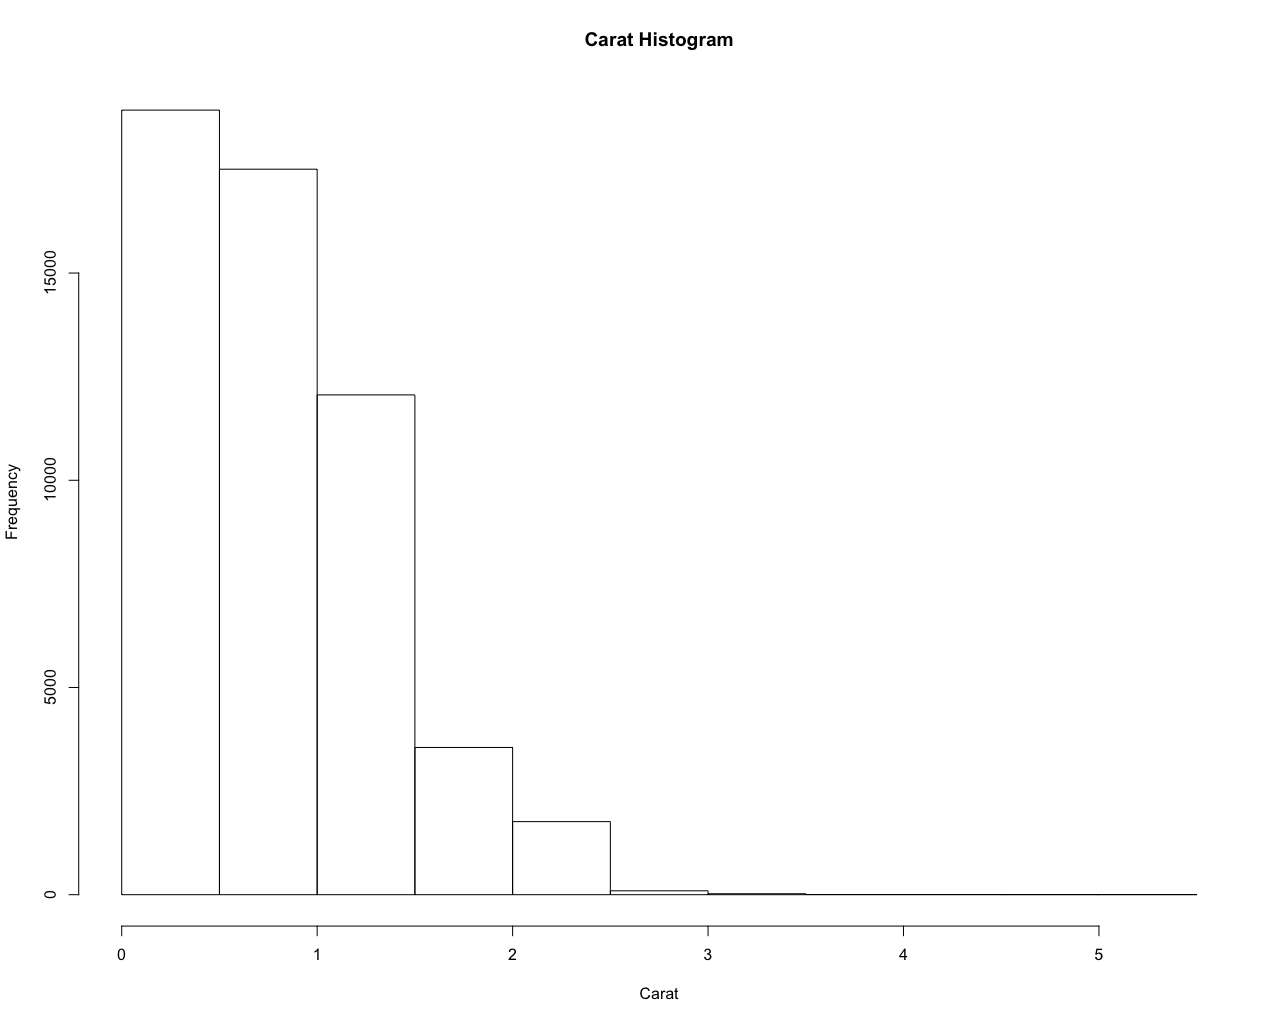
\includegraphics[width=\textwidth,height=0.75\textheight]{pic0021}\end{figure}
\end{frame}

\begin{frame}
\frametitle{Хистограма на каратите при 100 групи}
\begin{figure}[]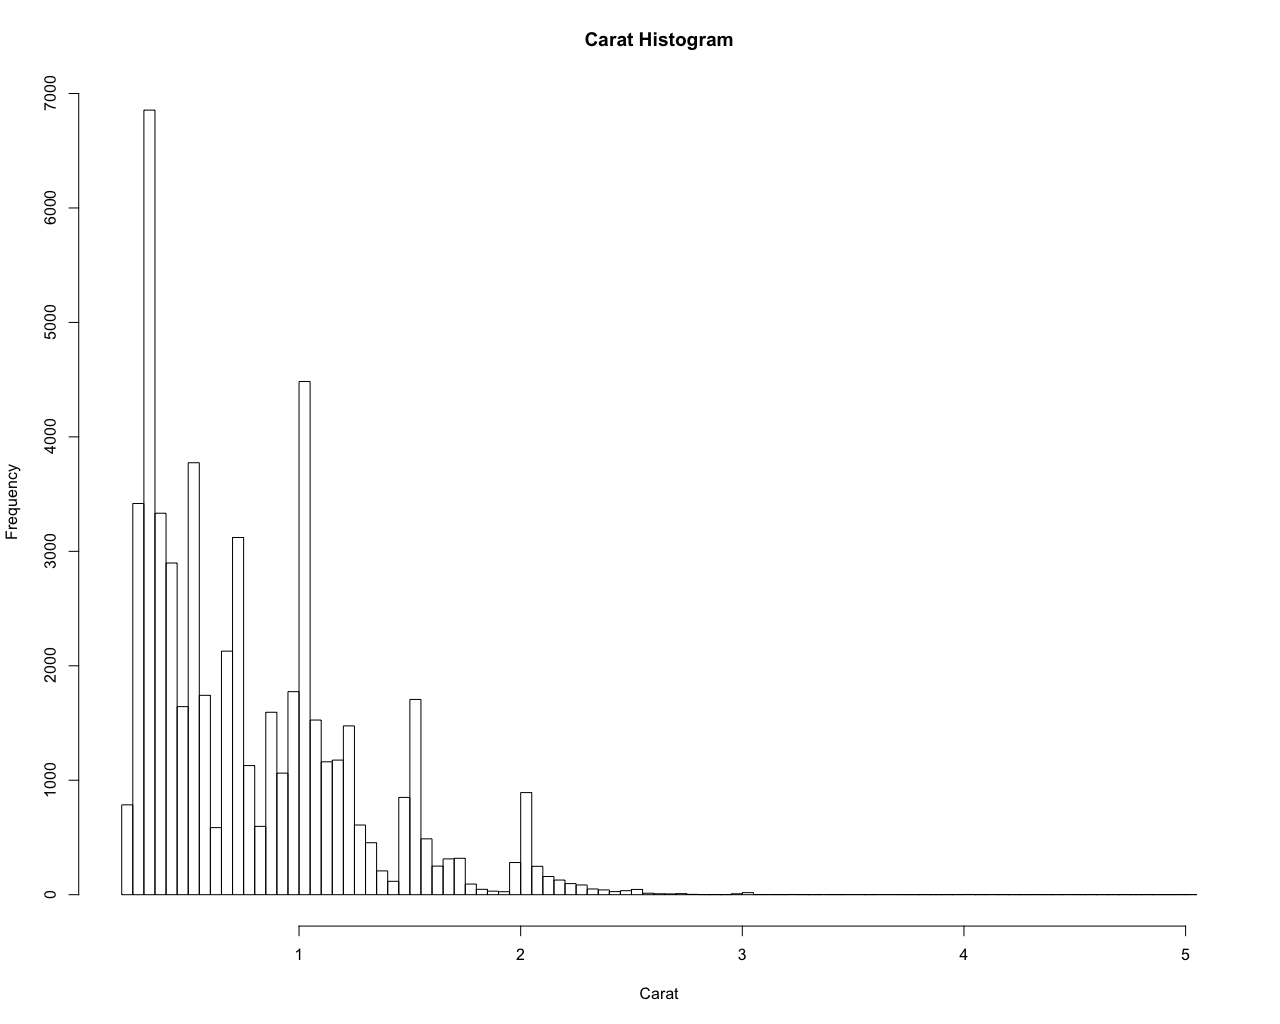
\includegraphics[width=\textwidth,height=0.75\textheight]{pic0022}\end{figure}
\end{frame}

\subsection{Диаграма на разсейване}

\begin{frame}
\frametitle{Отношение между два признака}
\begin{block}{Генериране на диаграма на разпръскване}
plot(price\textasciitilde carat, data=diamonds)
\end{block}

\begin{block}{Алтернативен запис}
plot(diamonds\$carat, diamonds\$price)
\end{block}
\end{frame}

\begin{frame}
\frametitle{Диаграма на разпръскване за камъните според отношението тегло към цена}
\begin{figure}[]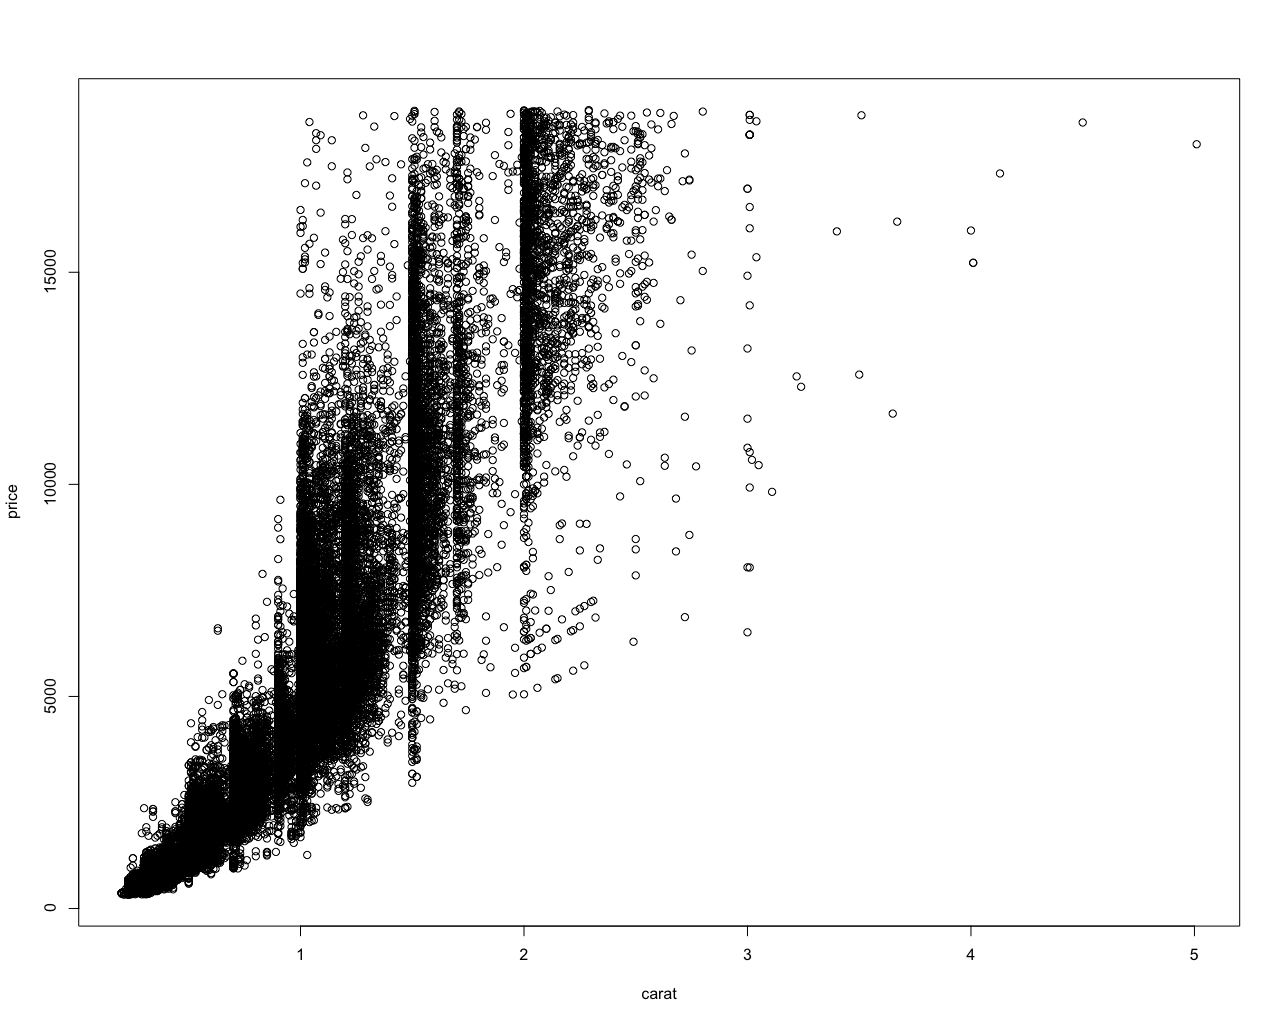
\includegraphics[width=\textwidth,height=0.75\textheight]{pic0023}\end{figure}
\end{frame}

\subsection{Графики тип кутия}

\begin{frame}
\frametitle{Квартили}
\begin{block}{Генериране на графика от тип кутия}
boxplot( diamonds\$carat )
\end{block}
\end{frame}

\begin{frame}
\frametitle{Графика тип кутия за теглото на диамантите}
\begin{figure}[]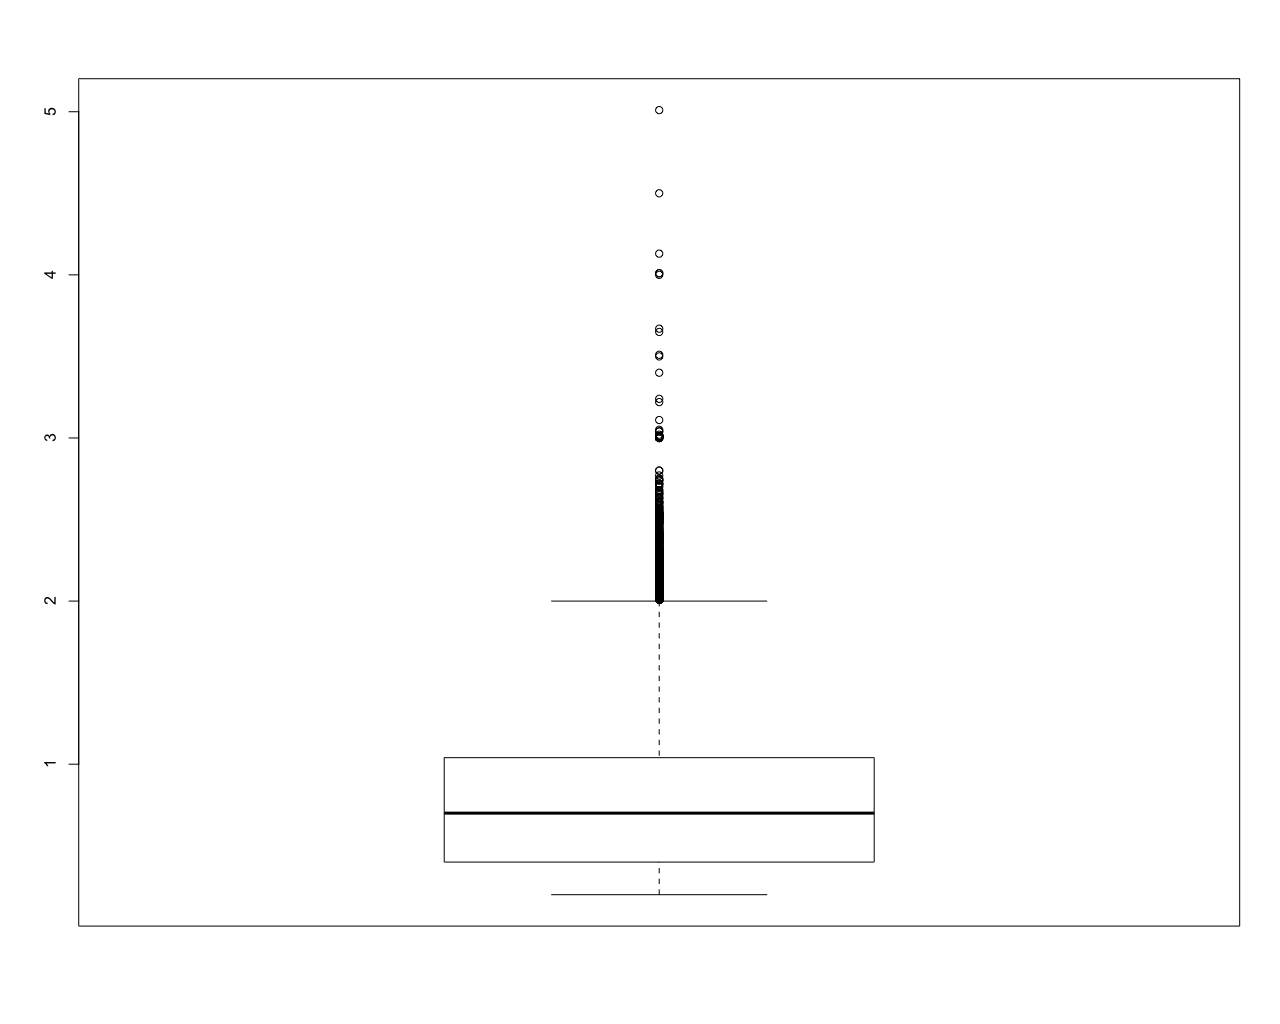
\includegraphics[width=\textwidth,height=0.75\textheight]{pic0024}\end{figure}
\end{frame}

\section{Заключение}

\begin{frame}
\center \huge{Заключение}
\end{frame}

\subsection{Дискусия}

\begin{frame}
\frametitle{Въпроси и отговори}
\center \huge{Благодаря за вниманието!}
\end{frame}

\end{document}
